\cotefile{10}
\scanpage{77}
quotient de $\handwritten{\overline}{\handwritten{\underline}{Q}}^{\handwritten{*}}$ par le sous-groupe des unités, donc canoniquement isomorphe à $\handwritten{\underline}{Q}$, par l'isomorphisme
\[
\handwritten{\overline}{\handwritten{\underline}{Q}}^{\handwritten{*}}/\text{unités}\handwritten{\longrightarrow}\handwritten{\underline}{Q}
\]
donnés par la valuation p-adique $v_p$, normalisée par la condition
\[
v_p(p)=1\quad .
\]
\unsure{A|L}'opération de $\deleted{\unsure{\pi_1(\underline{k}|\pi_1(\underline{K}|\pi(\underline{k}}}$ $\operatorname{Gal}(\handwritten{\overline}{\handwritten{\underline}{Q}}_p/\handwritten{\underline}{Q}_p)$ sur ce groupe quotient $Q$ est \unsure{triviale|trivialé|trivialè}, de sorte que $H$ est \handwritten{\uline}{diagonalisable} de groupe des caractères $\handwritten{\underline}{Q}$ :
\[
H=D(\handwritten{\underline}{Q})\quad .
\]
L'augmentation de Tate de $G$ correspond à l'homomorphisme
\[
\handwritten{\underline}{Z}\handwritten{\longrightarrow}\handwritten{\overline}{\handwritten{\underline}{Q}}^{\handwritten{*}},\quad 1\handwritten{\longmapsto}p\quad ,
\]
et l'augmentation induite sur $H$ correspond à l'\handwritten{\uline}{inclusion} canonique
\[
\handwritten{\underline}{Z}\handwritten{\lhook\joinrel\longrightarrow}\handwritten{\underline}{Q}
\]
(\unsure{grâee|grâce} à notre choix de la valuation \handwritten{\uline}{normalisée} comme indiquée).

\unsure{B|8}.2. Il faut maintenant expliciter l'homomorphisme de gerbes
\[
\handwritten{i:}\ \handwritten{\underline}{G}(\unsure{\handwritten{\underline}{F}|\handwritten{\underline}{\mathbb{F}}}_p)\handwritten{\longrightarrow}\handwritten{\underline{\Pi}}_p(\handwritten{\underline}{F}_p)
\tag*{\handwritten{(8.2.1)}}
\]
correspondant à l'inclusion
\[
i:\quad \handwritten{\underline}{Q}_p\text{-faisceaux constructibles}\handwritten{\lhook\joinrel\longrightarrow}\operatorname{Fcriso}(\handwritten{\underline}{F}_p)
\]
de 5.2. On a vu que l'image essentielle est exactement égale à la sous-catégorie \inserted{pleine} $J(\handwritten{\underline}{Q}_p\text{-faisceaux constructibles})$, \deleted{qui est} de sorte que $i$ s'identifie à une\deleted{foncteur} $\handwritten{\otimes}$-équivalence de la catégorie des $\handwritten{\underline}{Q}_p$-faisceaux constructibles avec elle-même. On constate alors que l'homomorphisme correspondant sur les liens $\deleted{\unsure{H\ H|H\to H}}$ $G'\handwritten{\longrightarrow}G'$ est l'identité, \deleted{et que} de sorte que $i$ est défini par un torseur sous $G'$, et que ce torseur sous $G'$ peut se décrire ainsi (aurait pu passer à la fin de 7, dans le cas d'un $k$ quelconque ...). On a un homomorphisme canonique
\[
\handwritten{\pi}_1(\handwritten{\underline}{F}_p^{\deleted{\handwritten{\unsure{*|\times}}}})=\handwritten{\hat}{\handwritten{\underline}{Z}}^{\deleted{\handwritten{\unsure{*|\times}}}}\handwritten{\longrightarrow}G'(\handwritten{\underline}{Q}_p),\quad \handwritten{\text{i.e. }(\pi_1(F_p))_{\mathbb{Q}_p}\longrightarrow G'}
\tag*{\handwritten{(8.2.2)}}
\]
d'où un \deleted{\unsure{homomorphi|homomorphix}} foncteur
\[
\text{torseurs}^{\deleted{\unsure{\underline{Q}_p|\underline{Q}_p\text{xxx}}}}\text{ sous }(\handwritten{\hat}{\handwritten{\underline}{Z}})_{\handwritten{\underline}{Q}_p}\handwritten{\longrightarrow}\text{torseurs sous }G'\ \deleted{\handwritten{\unsure{\xi|\varepsilon|,|.}}}\quad .
\]
% archive sheet number: 76
\scanpage{78}
D'autre part, on a un torseur évident $P_{\unsure{o|0}}$ sur $\handwritten{\underline}{Q}_p$ de groupe $(\handwritten{\hat}{\handwritten{\underline}{Z}})_{\inserted{\handwritten{\underline}{Q}_p}}$, correspondant à l'extension non ramifiée maximale de $\handwritten{\underline}{Q}_p$ ; on\deleted{t} prend l'image \inserted{$P$} de ce torseur: c'est lui.

8.3. Soit $\handwritten{\underline}{H}$ la gerbe noyau de (8.2.1), qui a donc comme lien le groupe diagonalisable $H$ de 8.1. D'après le sorite général (ref) la classe
\margin{\handwritten{$\underline{H}$ est aussi la \uline{gerbe des relèvements}, \uline{pour l'hom.}
\diagram{\begin{tikzcd}[ampersand replacement=\&,column sep=small,row sep=small]
j:\ \underline{G}(\unsure{F|\mathbb{F}}_p) \arrow[r] \arrow[d,phantom,"\simeq"{rotate=90}] \& \underline{\Pi}_p(F_p) \arrow[d,phantom,"\simeq"{rotate=90}] \\
[G] \& [G']
\end{tikzcd}}
déduit de l'hom $\unsure{G|\underline{G}}\longrightarrow G'$, du torseur $P$ ci-dessus.}}
\[
\handwritten{\xi\in}H^{\handwritten{2}}(\handwritten{\underline}{Q}_p,\deleted{\unsure{\underline{G}_m|G_m}}\ H)=\operatorname{Hom}(\handwritten{\underline}{Q},\operatorname{Br}(\handwritten{\underline}{Q}_p))=\operatorname{Hom}(\handwritten{\underline}{Q},\handwritten{\underline}{Q}/\handwritten{\underline}{Z})
\]
de cette gerbe est donnée par
\[
\handwritten{\xi=\unsure{\partial|\delta}(\unsure{\eta|\gamma})}
\]
où
\[
\handwritten{\eta\in}H^{\handwritten{1}}(\handwritten{\underline}{Q}_p,G')
\]
est la classe du torseur $P$. Pour faire le calcul, notons qu'on a un \deleted{sous-groupe}\inserted{quotient} $H'$ de $G_r$, correspondant au sous-groupe de $\deleted{\unsure{Q_p|\underline{Q}_p}}$ $\handwritten{\overline}{\handwritten{\underline}{Q}}_p^{\handwritten{*}}$ \deleted{formé} engendré par les raciens de l'unité(= éléments de torsion) et toutes les raciens de $p$, $p^{1/n}$ (ce groupe\deleted{\unsure{s|x}} est bien invariant par $\operatorname{Gal}(\handwritten{\overline}{\handwritten{\underline}{Q}}_p/\handwritten{\underline}{Q}_p)$ ). On a alors un homomorphisme d'extensions
\margin{\handwritten{\uline{NB} Ce diagramme est induit par un diagramme de \uline{gerbes} (valable sur un corps $k$ parfait quelconque) avec $\underline{H}'=$ gerbe correspondant \unsure{aux|à} la sous-catégorie de $\operatorname{Fcriso}(F_p)$ formé\unsure{e|s} des objets qui deviennent isomorphes sur une extension \uline{finie} $k'$ de $k=F_p$ à une somme d'objets $E_{r,s}$ ; et $H$ s'identifie à la \uline{gerbe des relèvements} de $P_o$ pour l'hom. $j:\underline{H}'\longrightarrow[\hat{\underline{Z}}]$ associé à $H'\longrightarrow(\hat{\underline{Z}})_{\mathbb{Q}_p}$ ...}}
\diagram{\begin{tikzcd}[ampersand replacement=\&]
0 \handwritten{\arrow[r]} \& H \handwritten{\arrow[r]} \handwritten{\arrow[d]} \& G \handwritten{\arrow[r]} \handwritten{\arrow[d]} \& G' \handwritten{\arrow[r]} \handwritten{\arrow[d]} \& 0 \\
0 \handwritten{\arrow[r]} \& H \handwritten{\arrow[r]} \& H' \handwritten{\arrow[r]} \& \handwritten{(\hat{\underline{Z}})_{\mathbb{Q}_p}} \handwritten{\arrow[r]} \& 0\ ,
\end{tikzcd}}
qui montre qu'on \deleted{\unsure{suffit de calculer|suffit de calculer xxx}} a
\[
\handwritten{\xi=\partial(\eta_o)},
\]
où
\[
\handwritten{\eta_o\in}H^{\handwritten{1}}(\handwritten{\underline}{Q}_p,\handwritten{\hat}{\handwritten{\underline}{Z}})
\]
est l'image de $\handwritten{\eta}$ par $G'\handwritten{\longrightarrow}\handwritten{\hat}{\handwritten{\underline}{Z}}$. On constate que le composé de (8.2.2) avec l'homomorphisme précédent est l'identité de $\handwritten{\hat}{\handwritten{\underline}{Z}}$, donc $\handwritten{\eta_o}$ est la classe du torseur canonique $P_o$ de la fin de 8.2. A l'aide\deleted{\unsure{x|s}} de ceci, il faut vérifier que la classe $\handwritten{\xi}$ correspond (par l'isomorphisme
\[
\operatorname{Br}(\handwritten{\underline}{Q}_p)\handwritten{\simeq}\handwritten{\underline}{Q}_{\deleted{\handwritten{\unsure{p|\ell}}}}/\handwritten{\underline}{Z}_{\deleted{\handwritten{\unsure{p|\ell}}}}
\]
du corps de classe local, à l'homomorphisme canonique $\handwritten{\mathbb{Q}\longrightarrow\mathbb{Q}/\mathbb{Z}}$
% archive sheet number: 77
\scanpage{79}
de \unsure{passgge|passsge|passage} au quotient (sauf erreur de signe, car je n'ai nulle part fait attention aux signes).

8.4. Considérons maintenant l'homomorphisme
\[
\handwritten{\underline}{G}(\handwritten{\overline}{\unsure{\handwritten{\underline}{F}|\handwritten{\underline}{\mathbb{F}}}}_p)\handwritten{\longrightarrow}\handwritten{\underline}{G}(\handwritten{\underline}{F}_p)\quad .
\tag*{(8.4.1)}
\]
Il est clair qu'il se factorise par $\handwritten{\underline}{H}$ (i.e. que le composé
\[
\handwritten{\underline}{Q}_p\text{-faisceaux constructibles sur }\handwritten{\underline}{F}_p\ \overset{i}{\handwritten{\longrightarrow}}\ \operatorname{Fcriso}(\handwritten{\underline}{F}_p)\handwritten{\longrightarrow}\operatorname{Fcriso}(\handwritten{\overline}{\handwritten{\underline}{F}}_p)
\]
s'envoie dans les objets ``constants'' ...) , d'où un homomorphisme
\[
\handwritten{\underline}{G}(\handwritten{\overline}{\handwritten{\underline}{F}}_p)\handwritten{\longrightarrow}\handwritten{\underline}{H}\quad .
\tag*{(8.4.2)}
\]
Par Dieudonné-Manin, on connait la structure des objets de $\operatorname{Fcriso}(\handwritten{\overline}{k})$ pour $\handwritten{\overline}{k}$ algébriquement clos\deleted{\unsure{x|e}}, on sait que ces objets sont semi-simples et proviennent (mod isomorphisme) d'objets de $\operatorname{Fcriso}(\handwritten{\underline}{F}_p)$. Cela implique que (8.4.1), donc aassi (8.4.2), est un monomorphisme de gerbes. Pour montrer que c'est une équivalence, il suffit de montrer qu'un objet simple non constant de \deleted{$\handwritten{\underline}{H}$ me donne} $\operatorname{Rep}(\handwritten{\underline}{H})$ donne un objet non constant de $\operatorname{Rep}(\handwritten{\underline}{G}(\handwritten{\overline}{k}))\handwritten{\overset{\approx}{\longrightarrow}}\operatorname{Fcriso}(\handwritten{\overline}{k}))$. Or les \unsure{cla sees|cla ses|classes} d'objetssimples de $\operatorname{Rep}(\handwritten{\underline}{H})$ sont indexés par les éléments de $\handwritten{\underline}{Q}$, et si on considère l'objet simple de $\operatorname{Fcriso}(\handwritten{\underline}{F}_p)\handwritten{\simeq}\operatorname{Rep}(\handwritten{\underline}{G}(\handwritten{\underline}{F}_p^{\deleted{\handwritten{\unsure{*|\overline{\vphantom{F}}}}}}))$ défini par $(E,\handwritten{\underline}{F}_E)$, avec $\handwritten{\underline}{F}_E$ ayant comme polynôme minimal $T^r-p^s$ avec $r,s\handwritten{\in}\handwritten{\underline}{Z}$, $r\geq1$, $(r,s)=1$, alors sa restriction à $\handwritten{\underline}{H}$ donne un objet simple \deleted{\unsure{de|du}} (car il reste simple dans $\operatorname{Fcriso}(\handwritten{\overline}{k})$) de classe $s/r\handwritten{\in}\handwritten{\underline}{Q}$, et celui\handwritten{-}ci, d'après la classification de Dieudonné-Manin, \deleted{n'est pas} a une image dans $\operatorname{Fc\ iso}(\handwritten{\overline}{k})$ qui n'est pas constante si $r\handwritten{\ne}0$ ...

\handwritten{8.5.} On a donc \deleted{déterminé} résolu par l'affirmative, pour $k=\handwritten{\underline}{F}_p$, la question 6.2, en déterminant en même temps (à équivalence définie à isomorphisme unique près) la gerbe $\unsure{\handwritten{\underline}{G}|\handwritten{\underline}{H}}(\handwritten{\overline}{k})$ associée à une clôture algébrique $\handwritten{\overline}{k}$ de $k=\handwritten{\underline}{F}_p$ ; \deleted{comme pour} elle ne dépend pas (à \deleted{\unsure{isomorphi|isomorphix}} équivalence déterminée à isomorphisme unique près) du choix de la clôture algébrique envisagée $\handwritten{\overline}{k}$, et par Dieudonné-Manin est can. équi%
% archive sheet number: 78
\scanpage{80}%
valente à $\handwritten{\underline}{G}(\handwritten{\unsure{\ell|\gamma}})$ pour tout corps alg. clos $\handwritten{\ell}$ de car\deleted{\unsure{r|.}}. $p\handwritten{>0}$ (de façon précise, si $\handwritten{\overline}{\unsure{\handwritten{\underline}{F}|\handwritten{\underline}{\mathbb{F}}}}_p$ est\deleted{\unsure{x|t}} la clôture algébrique de $\handwritten{\underline}{F}_p$ dans $\handwritten{\ell}$, l'inclusion de celle-ci dans $\handwritten{\ell}$ induit une équivalence de gerbes
\[
\handwritten{\underline}{G}(\handwritten{\ell})\handwritten{\underline{\approx}}\handwritten{\underline}{G}(\handwritten{\overline}{\handwritten{\underline}{F}}_p)\deleted{\handwritten{\unsure{)|,}}}\handwritten{\underline{\approx}}\handwritten{\underline}{H}\deleted{\handwritten{\unsure{)|.}}}\qquad ).
\]
8.6. Etude de $\operatorname{Rep}(\handwritten{\underline}{H})$. Nous avons dit que les classes d'objets simples sont en correspondance biunivoque avec les éléments de $\handwritten{\underline}{Q}$ ; l'élément de $\handwritten{\underline}{Q}$ correspondant à un objet isotypique est dit la \handwritten{\uline}{pente} de cet élément. Nous avons vu que l'objet de $\operatorname{Rep}(\handwritten{\underline}{H})$ défini \margin{\handwritten{Notation $E_{s/r}$ pour $E_{r,s}$ indiquée, donc
\[
E_\lambda\otimes E_{\lambda'}\simeq E_{\lambda\lambda'}^{n(\lambda,\lambda')}
\]
pour $\lambda,\lambda'\in\mathbb{Q}$}}
par l'objet $\handwritten{\underline}{Q}_p[T]/(T^r-p^s)$ de $\operatorname{Fcriso}(\handwritten{\underline}{F}_p)$, muni de la multiplication par $T$, est simple de pente $s/r$ ($s,r\handwritten{\in}\handwritten{\underline}{Z}$, $r\geq1$, $(s,r)=1$ ), de sorte que nous obtenons ainsi un catalogue complet des objets simples $E_{r,s}$. Bien entendu, $E_{r,s}$ est de rang $r$, d'autre part son corps des endomorphismes est \deleted{\unsure{il|ila}} un corps gauche \inserted{$K_{r,s}$} dont la classe dans $\operatorname{Br}(\handwritten{\underline}{Q}_p)=\handwritten{\underline}{Q}/\handwritten{\underline}{Z}$ est $s/r\bmod1$, d'après ce qu'on a vu dans 8.3.

$\operatorname{Rep}(\handwritten{\underline}{H})$ est limite inductive des sous-catégories pleines $\operatorname{Rep}(\handwritten{\underline}{H},r)$, $r\geq1$, où $(\handwritten{\underline}{H},r)$ est le quotient de la gerbe $\handwritten{\underline}{H}$ correspond au quotient $(H,r)\handwritten{\simeq}\handwritten{\underline}{G}_m$ de son lien, tel que l'homomorphisme de Tate \deleted{\unsure{soit un|soitxxx}} induise un homomorphisme $(H,r)\handwritten{\xrightarrow{\unsure{a|q|\alpha}}}\handwritten{\underline}{G}_m$ s'identifiant à $x\handwritten{\longmapsto}x^r$ : F-iso\inserted{cristaux (sur $\handwritten{\overline}{k}$) de pente multiple de $1/r$.} Donc $(\handwritten{\underline}{H},r)$ \deleted{\unsure{s'identifie}} èst\deleted{\unsure{x|à}} \inserted{une} gerbe de lien $\handwritten{\underline}{G}_m$, ayant comme classe dans $\operatorname{Br}(\handwritten{\underline}{Q}_p)$ le générateur canonique $1/r\bmod\handwritten{\underline}{Z}$ de ${}_r\operatorname{Br}(\handwritten{\underline}{Q}_p)\handwritten{\simeq}\handwritten{\underline}{Z}/r\handwritten{\underline}{Z}$. C\unsure{,'|'}est aussi, plus canoniquement, ``la'' gerbe définie par le corps gauche $K_{r,\handwritten{1}\deleted{\unsure{s|1}}}$ plus haut, \deleted{qui}

\handwritten{[}Exercice amusant, que je n'ai pas fait: la structure additive de $\operatorname{Rep}(\handwritten{\underline}{H})$ étant entièrement décrite par la collection des $K_{r,s}$, expliciter sa $\handwritten{\otimes}$-structure ... i.e. écrire les \handwritten{``}relations canoniques\handwritten{''} en termes de prod\unsure{u|n}i\unsure{t|e}s tensoriels entre les $E_{r,s}$. Autre exerciee suggéré: trouver ``canoniquement'' une description des modules de Dieudonné des réduits des groupes de Lubin-Tate en termes des $E_{r,s}$ \deleted{\handwritten{\unsure{,|.}}} \handwritten{(}en particulier, les Lubin-Tate associés aux extensions non ramifiées
% archive sheet number: 79
\scanpage{81}
de $\handwritten{\underline}{Q}_p$ \handwritten{)} qui sont donc isomorphes \inserted{\handwritten{``géométriquement'' i.e. dans $\operatorname{Rep}(\underline{H})$}} (mais sans doute non canoniquement) aux $E_{r,1}$ pour $r\geq1$: ils donnent des modules libres de rang 1 canoniques sous les $K_{r,1}$ ...\handwritten{]}

9. Pour $k$ quelconque, on trouve un \deleted{ho} $\handwritten{\otimes}$-homomorphisme canonique \deleted{(à l'aide} défini à isomorphisme unique près (on utilise un choix d'une clôture algébrique $\handwritten{\overline}{k}$ de $k$, mais ce choix est inessentiel ..)
\[
\operatorname{Fcriso}(k)\handwritten{\longrightarrow}\operatorname{Rep}(\handwritten{\underline}{H})
\]
ou encore un homomorphisme de gerbes
\[
\handwritten{\underline}{H}\handwritten{\longrightarrow}\handwritten{\underline}{G}(k)
\]
(rappelons que cet homomorphisme se factorise par le noyau,\deleted{de} soit \deleted{\unsure{G|Gr}} $\handwritten{\underline}{H}(k)$, de $\handwritten{\underline}{G}(k)\handwritten{\to}\handwritten{\underline{\Pi}}_p(k)$, et que pour $k$ parfait on devine que l'homomorphisme obtenu $\handwritten{\underline}{H}\handwritten{\to}\handwritten{\underline}{H}(k)$ est une équivalence ...). Si $\handwritten{\lambda\in}\handwritten{\underline}{Q}$, un F\deleted{(}\handwritten{-}isocristal sur $k$ est dit \deleted{\unsure{homogèn|homogène}} \handwritten{\uline}{de pente} $\handwritten{\lambda}$ si son image dans $\operatorname{Rep}(\handwritten{\underline}{H})$ est de pente $\handwritten{\lambda}$. On voit alors aussitôt qu'un F-isocristal est de pente zéro sss il est ``trivial'' i.e. satisfait aux conditions de 5.2 (ce qui justifie la terminologie qui est introduite, un peu prématurément, à cet endroit), il est effectif sss son image dans \inserted{$\operatorname{Rep}(H)$ l'est,i.e. est à pente $\handwritten{\geq}$ 0.}

Considérons l'homomorphisme de liens associé
\[
H\handwritten{\longrightarrow}G(k)\quad ,
\]
on trouve \unsure{alons|alors} que si $k$ est parfait, l'homomorphisme précédent est \handwritten{\uline}{central}, en d'autres termes $H$ opère sur le foncteur identique de $\operatorname{Fcriso}(k)\handwritten{\to}\operatorname{Rep}(\handwritten{\underline}{G}(k))$, de sorte que tout F-isocristal \inserted{$(E,F_E)$} se décompose en ses \handwritten{``}\handwritten{\uline}{composantes isopentiques}\handwritten{''} $E_{\handwritten{\lambda}}$, $\handwritten{\lambda\in}\handwritten{\underline}{Q}$. $E$ est ``trivial'' resp. effectif sss $E_{\handwritten{\lambda}}=0$ pour $\handwritten{\lambda\ne}$ 0 (resp. $\handwritten{\lambda<0}$).

Notons que le \inserted{F-iso}cristal de Tate $K(\unsure{1|l})$ est de pente\handwritten{-}1. Donc (pour $k$ parfait) tout F\deleted{(}\handwritten{-}isocristal se met de façon unique sous la forme
\[
E=\handwritten{\sum_{i\in\mathbb{Z}}}E_i(-i)\quad ,
\]
où $E_i$ est à composantes isopentiques de pente $0\handwritten{<}\,\inserted{\handwritten{i}}\handwritten{\leq}1$. D'ailleurs,
% archive sheet number: 80
\scanpage{82}
les $E_i$ qui sont à composantes \unsure{isopyptiques|isopentiques|isopyntiques|isopypiques|isotypiques} $\handwritten{\lambda}$ tels que $0\handwritten{<\lambda\leq\unsure{<}}1$ sont exactement les modules de Dieudonné des groupes formels $p$-divisibles sur $k$ (la catégorie de ces modules de Dieudonné \deleted{correspond à}\inserted{est opposée à} la catégorie de ces groupes, mod isogénie). D'autre part, un F-isocristal est d'amplitude isopentique contenue dans $\handwritten{[}0,1\handwritten{]}$ (intervalle fermé) sss c'est le module de Dieudonné d'un groupe de Barsotti-Tate sur $k$ (la catégorie des F-isocristaux envisagée étant \inserted{anti}équivalente à la catégorie des groupes de B.T. sur $k$ mod. isogénie ..): le F-isocristal unité correspond au groupe de B.T. ind-étale $\handwritten{\underline}{Q}_p/\handwritten{\underline}{Z}_p$ sur $k$.

Supposant toujours $k$ parfait, la condition \deleted{de l'existe} que $(E,F_E)$ soit effectif èt qu'il existe un $V_i$ \inserted{effectif} tel que $FV_i=V_iF=p^i\operatorname{id}$ (cf n\textsuperscript{o}2) signifie que $E$ est d'amplitude isopentique contenue dans $\handwritten{[}0,i\handwritten{]}$.

10. \handwritten{\uline}{Cas} $k$ \handwritten{\uline}{fini}. Supposons $k={\unsure{\handwritten{\underline}{F}|\handwritten{\underline}{\mathbb{F}}}}_q^{\deleted{\handwritten{\unsure{*|\overline{\vphantom{F}}}}}}$, où $q=p^{\deleted{a}\handwritten{\unsure{\nu|a}}}$. En vertu de 6.1, \deleted{son} la gerbe $\handwritten{\underline}{G}(\handwritten{\underline}{F}_q)$ est connue, c'est la sous-gerbe évidente de $\handwritten{\underline}{G}(\handwritten{\underline}{F}_p)$, s'insérant dans une suite exacte
\[
0\handwritten{\longrightarrow}\handwritten{\underline}{G}(\handwritten{\underline}{F}_q)\handwritten{\longrightarrow}\handwritten{\underline}{G}(\handwritten{\underline}{F}_p)\handwritten{\longrightarrow}\operatorname{Rep}(\handwritten{\underline}{Z}/\deleted{a}\handwritten{\nu}\handwritten{\underline}{Z})\handwritten{\longrightarrow}0\quad .
\]
Il est clair alors que pour $\handwritten{\underline}{F}_q$ comme pour $\handwritten{\underline}{F}_p$, la réponse à 6.2 est affirmative, donc les considérations du n\textsuperscript{o}7 s'appliquent: on trouve la structure de $\handwritten{\underline}{G}(\handwritten{\underline}{F}_q)$ comme gerbe + ses structures supplémentaires examinées jusqu'à présent.

Le foncteur fibre \inserted{canonique $(E,F_E)\handwritten{\longmapsto}E$} sur $\operatorname{Fcriso}(\handwritten{\underline}{F}_q)$ \deleted{à valeur} sur le corps $K_{\deleted{a}\handwritten{\nu}}=K(\handwritten{\underline}{F}_{q=p^{\deleted{a}\handwritten{\nu}}})$ \margin{\handwritten{\unsure{présenter|préciser} plutôt $f_q$ comme un \uline{autom. du foncteur identique} de $\operatorname{Fcriso}(F_q)$, donne un élément de $G_\nu(\mathbb{Q}_p)$}}
(i.e. section canonique de $\handwritten{\underline}{G}(\handwritten{\underline}{F}_q)$ sur $K_{\deleted{a}\handwritten{\nu}}$) est muni d'une structure supplémentaire, savoir un automorphisme linéaire $F_E{}^a$, de sorte que le groupe \deleted{algébrique} sur \deleted{k} $K_a$ correspondant à cette section de $\handwritten{\underline}{G}(\handwritten{\underline}{F}_q)$ sur $K_a$, savoir le sous-groupe \inserted{$\handwritten{G_\nu=\nu}$}$\deleted{a}.G_{\deleted{K_a}\handwritten{K_\nu}}$ de $G_{K_{\deleted{a}\handwritten{\nu}}}$ ouvert d'indice $\deleted{a}\handwritten{\nu}$ (correspondant au sous-groupe des racines $\deleted{a}\handwritten{\nu}$.èmes de 1 dans le groupe des caractères $\handwritten{\overline}{\handwritten{\underline}{Q}}^{\handwritten{*}}$ de $G_{\handwritten{K_\nu}}$)

% archive sheet number: 81
\scanpage{83}
est muni d'un élément \inserted{$\handwritten{\underline}{f}_q$} de $G_{\deleted{a}\handwritten{\unsure{\nu|a}}}(K_{\deleted{a}\handwritten{\nu}})$\inserted{(\handwritten{``}Frobenius relatif à $\unsure{\handwritten{\underline}{F}|\handwritten{\underline}{\mathbb{F}}}_q$'')}. Ce dernier n'est autre d'ailleurs que $\deleted{\handwritten{\underline}{f}_q}$ $\handwritten{\underline}{f}^{\deleted{a}\handwritten{\nu}}$, où $\handwritten{\underline}{f}$ est le générateur canonique de $G$ (le Frobenius absolu \handwritten{!}). \deleted{\unsure{O|C} on voit donc que $G_a$ est encore engendré par} Notons que $a\unsure{\operatorname{Id}|\operatorname{id}}_G$ est un monomorphisme (car $x\handwritten{\mapsto}x^{\deleted{a}\handwritten{\nu}}$ est un épimorphisme dans $\handwritten{\overline}{\handwritten{\underline}{Q}}_{\handwritten{p}}^{\handwritten{*}}$ ), donc induit un isomorphisme entre $G_{K_{\deleted{a}\handwritten{\nu}}}$ et $G_{\deleted{a}\handwritten{\nu}}\handwritten{\simeq}G(\handwritten{\underline}{F}_q)$,transformant le frobenius \deleted{\unsure{relati|relatif}} absolu en le frobenius relatif à $\handwritten{\underline}{F}_q$. Grâce à ceci, on voit :

\handwritten{\uline}{Proposition} 10.1. La catégorie \inserted{tann.} $\operatorname{Fcriso}(\handwritten{\underline}{F}_q)\handwritten{\otimes}_{\handwritten{\underline}{Q}_p}K_a$ est équivalente à la catégorie \inserted{tann.} $\operatorname{Fcriso}(\handwritten{\underline}{F}_p)\handwritten{\otimes}_{\handwritten{\underline}{Q}_p}K_a$,\deleted{\handwritten{\unsure{(|/}}} \margin{\handwritten{(i.e. la catégorie des couples $(E,F'_E)$ d'un vectoriel sur $K_\nu$ et d'un autom. de ce vectoriel....)}}
avec $\handwritten{\underline}{f}_q$ correspondant à $\handwritten{\underline}{f}^{\deleted{a}\handwritten{\nu}}$ (où on peut, si on veut, considérer $\handwritten{\underline}{f}_q$ et $\handwritten{\underline}{f}$ comme des endomorphismes des foncteurs identiques de $\operatorname{Fcriso}(\handwritten{\underline}{F}_q)$ resp. $\operatorname{Fcriso}(\handwritten{\underline}{F}_p)$)), et correspondance des foncteurs fibres canoniques. Le foncteur déduit du changement de base $\handwritten{\underline}{F}_p\handwritten{\to}\handwritten{\underline}{F}_q$

\[
\operatorname{Fcriso}(\handwritten{\underline}{F}_p)\handwritten{\otimes}_{\handwritten{\underline}{Q}_p}K_{\deleted{a}\handwritten{\nu}}\handwritten{\longrightarrow}\operatorname{Fcriso}(\handwritten{\underline}{F}_q)\handwritten{\otimes}_{\handwritten{\underline}{Q}_p}K_{\deleted{a}\handwritten{\nu}}
\]
s'identifie, par l'équivalence précédente, au foncteur qui à tout couple $(E,F_E)$ d'un vectoriel sur $K_{\deleted{a}\handwritten{\nu}}$ et d'un automorphisme dudit, associe le couple $(E,F_E{}^{\deleted{a}\handwritten{\nu}})$\handwritten{;}
\inserted{\handwritten{analogue pour $\operatorname{Fcriso}(F_{\unsure{q|1}})-\operatorname{Fcriso}(F_q)\otimes_{\mathbb{Q}_p}K_\nu$, il s'identifie : $(E,F_E)\longmapsto(E,F_E{}^\nu)$.}}

10.2. Comme on connait $\handwritten{\underline}{G}(\handwritten{\underline}{F}_q)$ comme une sous-gerbe $\handwritten{\underline}{G}_{\deleted{a}\handwritten{\nu}}$ de $\handwritten{\underline}{G}=\handwritten{\underline}{G}(\handwritten{\underline}{F}_p)$, et que celle-ci contient $\handwritten{\underline}{H}$, on connait donc en principe l'inclusion
\[
\handwritten{\underline}{H}\handwritten{\longrightarrow}\handwritten{\underline}{G}_{\deleted{a}\handwritten{\nu}}=\handwritten{\underline}{G}(\handwritten{\underline}{F}_q)\quad ,
\]
donc aussi le foncteur
\[
\operatorname{Rep}(\handwritten{\underline}{G}_{\deleted{a}\handwritten{\nu}})\handwritten{\simeq}\operatorname{Fcriso}(\handwritten{\underline}{F}_q)\handwritten{\longrightarrow}\operatorname{Rep}(\handwritten{\underline}{H})\quad ,
\]
\deleted{\inserted{et} Considérons le foncteur correspondant}
\[
\deleted{\operatorname{Fcriso}(\handwritten{\underline}{F}_q)\handwritten{\otimes}_{\handwritten{\underline}{Q}_p}K_{\underset{\deleted{\unsure{a|x}}}{a}}\quad\operatorname{Rep}(\handwritten{\underline}{H})\handwritten{\otimes}_{\handwritten{\underline}{Q}_p}K_a\ .}
\]
L'effet de ce\deleted{s} foncteur\deleted{s} sur les classes d'isomorphie d'éléments est connu (comme chaque fois qu'il s'agit d'un morphisme d'une \deleted{gerbe de} \unsure{Catégorie|catégorie|Oatégorie} tannakienne à lien commutatif dans une autre à lien de type multiplicatif) par la connaissance de l'homomorphisme de liens correspondant
% archive sheet number: 82
\scanpage{84}
\diagram{\begin{tikzcd}[ampersand replacement=\&]
H \handwritten{\arrow[r,"\handwritten{u_\nu}"]} \& G_{\handwritten{\nu}}\ \handwritten{(} \handwritten{\arrow[r]} \& G\handwritten{)}\ ,
\end{tikzcd}}
lui-même déterminé par la connaissance de l'homomorphisme en sens inverse sur les groupes de caractères
\diagram{\begin{tikzcd}[ampersand replacement=\&]
Q \& \handwritten{\overline}{\handwritten{\underline}{Q}}^{\handwritten{*}} \handwritten{\arrow[l,"\handwritten{u_\nu^*}"']} \& \handwritten{\overline}{\handwritten{\underline}{Q}}^{\handwritten{*}} \handwritten{\arrow[l,"\handwritten{\lambda^\nu}"']} \handwritten{\arrow[ll,bend left=25,"\handwritten{|\lambda|}"']}\quad .
\end{tikzcd}}
On lit sur ce diagramme que, pour l'isomorphisme naturel du groupe des caractères de $G_{\handwritten{\nu}}$ avec $\handwritten{\overline}{\handwritten{\underline}{Q}}^{\handwritten{*}}$, provenant de l'élément $\handwritten{\underline}{f}_q\handwritten{\in}G_{\handwritten{\nu}}(\handwritten{\underline}{Q})$, \handwritten{on} \deleted{qui donne}\inserted{\handwritten{a}}
\[
u_{\handwritten{\nu}}^{\handwritten{*}}(\handwritten{\lambda})=v_p(\handwritten{\lambda})/\handwritten{\nu}\quad .
\]
On trouve donc\deleted{x} le résultat suivant de Manin, énoncé sous une forme plus jolie et débaréssé d'hypothèses restrictives parasites:

\handwritten{\uline}{Proposition} 10.3. Soit $(E,F_E)$ un F-isocristal sur $\unsure{\handwritten{\underline}{F}|\handwritten{\underline}{\mathbb{F}}}_q$, $q=p^{\handwritten{\nu}}$, et considérons le polynôme ca\unsure{\handwritten{r}|r}actéristique $f(T)$ de $F_E{}^{\handwritten{\nu}}$, \margin{\handwritten{NB si on prend plutôt la val. $\unsure{v_q|\nu_q}$ telle que $v_q(q)=1$, on trouve les valeurs propres $v_q(\lambda_i)$ (sans diviser par $\nu$)}}
soient $\handwritten{\lambda}_1,..,\handwritten{\lambda}_N$ ($N=\operatorname{rang}E$) ses racines, et $c_1$ , $..,c_{\handwritten{N}}$ leurs valeurs absolues normalisées ($c_i=v_p(\handwritten{\lambda}_i)$, $v_p(p)=1$). Alors \deleted{sur} dans $\operatorname{Rep}(\unsure{\handwritten{\underline}{H}|\handwritten{\underline}{G}})\handwritten{\otimes}_{\handwritten{\underline}{Q}_p}\handwritten{\overline}{\handwritten{\underline}{Q}}_p\handwritten{\simeq}\unsure{\operatorname{Fcriso}|\operatorname{Ecriso}}(\handwritten{\overline}{\handwritten{\underline}{F}}_q)\handwritten{\otimes}_{\handwritten{\underline}{Q}_p}\handwritten{\overline}{\handwritten{\underline}{Q}}_p$, l'image de $(E,E_E)$ a comme pentes les nombres $c_1/\handwritten{\nu}$, $...$ $c_N/\handwritten{\nu}$, de sorte que, si les \inserted{différentes} pentes possibles sont $\deleted{p_i}$\deleted{ avec multiplicité} $p_i=s_i/r_i$ ($s_i,r_i\handwritten{\in}\handwritten{\underline}{Z}\deleted{\unsure{x|r}}$, $r_i\handwritten{\geq}1$, $(s_i,r_i)=1$) \deleted{\handwritten{$\unsure{d_ip_i\in Q|d_i,p_i\in Q|d_ip_i\in Z|d_i,p_i\in Z}$}} avec multiplicité $d_i$, on a $r_i\handwritten{\mid}d_i$ i.e\handwritten{,} $d_i=d'_ir_i$, et l'image de $(E,F_E)$ dans $\operatorname{Fcriso}(\handwritten{\overline}{\handwritten{\underline}{F}}_p)$ est isomorphe à $\handwritten{\sum_i}E_{p_i}^{d'_i}$.


\handwritten{\uline{Cor.}}
% archive sheet number: 83

\scanpage{86}
\mspage{\handwritten{18}}
\mspage{\deleted{\handwritten{\unsure{16|18}}}}
\margin{\handwritten{\figure{\begin{tikzpicture}[x=.12cm,y=.12cm]
\draw[line width=.6pt] (0,1.55)--(-.04,1.25);
\draw[line width=.4pt] (-.08,.8)--(-.12,-.2);
\end{tikzpicture}}}}
2.7\handwritten{\unsure{.|!}} \handwritten{\uline}{Topos classifiant d'un \inserted{\handwritten{pro-}}groupe \deleted{profini}.}

\handwritten{2.7.1} Soit $\inserted{\handwritten{\underline}{G}=}(G_i)_{i\handwritten{\in}I}$ un systême projectif \deleted{strict} de groupes, avec $G_i,I\handwritten{\in}\handwritten{\underline}{U}$. On suppose le systême projectif \handwritten{\uline}{strict}, i.e. les morphismes de transition $G_j\handwritten{\to}G_i$ surjectifs. \margin{\handwritten{\figure{\begin{tikzpicture}[x=.3cm,y=.3cm]
\draw (0,.15) .. controls (.2,-.05) and (.4,-.25) .. (.65,-.2);
\end{tikzpicture}}}}Si $E$ est un ensemble, on \deleted{dit que $G$ opère sur $E$} \deleted{si} appelle \handwritten{\uline}{opération de} $\handwritten{\underline}{G}$ \handwritten{\uline}{sur} $E$\inserted{(à gauche, disons)} la structure suivante: a) une famille $(E_i)_{i\handwritten{\in}I}$ de parties de $E$, de réunion $E$; b) pour tout $i\handwritten{\in}I$, une opération du groupe $G_i$ sur l'ensemble $E_i$ ; on suppose de plus ces données soumises à la condition suivante: pour $j\handwritten{\geq}i$, $E_i$ est le sous-ensemble de $E_j$ formé des éléments fixes sous le groupe noyau de $G_j\handwritten{\to}G_i$. On dit \inserted{\handwritten{aussi}} que \handwritten{\uline}{$G$ opère sur} $E$ (à gauche) si on s'est donnée\deleted{\unsure{s|x}} une opération de $G$ sur $E$ (à gauche).

Les ensembles $\handwritten{\in}\handwritten{\underline}{U}$ munis d'une opération de $\handwritten{\underline}{G}$ forment une catégorie de façon évidente. On constate aussitôt, grâce au critère de Giraud, que cette catégorie est un \inserted{\handwritten{$\underline{U}$-}}topos. On le note $B_{\handwritten{\underline}{G}}$ et on llappel\unsure{\deleted{l}|\handwritten{l}|l\handwritten{/}}e \handwritten{\uline}{topos classifiant de $G$}. Lorsque $I$ admet un objet \deleted{\unsure{fin|fix}} initial $i_{\unsure{o|0}}$, posant $G=G_{i_o}$, on retrouve le topos classifiant de 2.3.
\margin{\handwritten{\figure{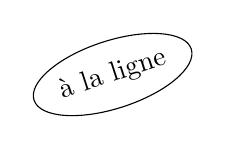
\begin{tikzpicture}[baseline]
\draw[rotate=18] (0,0) ellipse (1.05 and .43);
\node[rotate=18] at (0,0) {à la ligne};
\end{tikzpicture}}}}

\handwritten{\figure{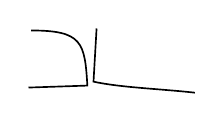
\begin{tikzpicture}[x=.65cm,y=.5cm]
\draw[line width=.6pt] (-1.1,.8) .. controls (-.1,.8) and (-.05,.5) .. (0,-.6) -- (-1.15,-.65);
\draw[line width=.6pt] (.18,.85)--(.12,-.5) .. controls (.65,-.65) and (1.4,-.68) .. (2.1,-.78);
\end{tikzpicture}}}
\inserted{\handwritten{2.7.2.}} Un autre exemple important est celui où les groupes $G_i$ sont finis, de sorte que
\[
G=\underset{\handwritten{\longleftarrow}}{\lim}G_i
\]
est\deleted{\unsure{n|x}} un groupe topologique compact totalement discontinu, ou \handwritten{\uline}{groupe profini}. Une opération de $\handwritten{\underline}{G}$ sur $E$ revient alors à une opération de $G$ sur $E$ qui est continue, ou ce qui revient au même, telle que le stabilisateur de tout point de $E$ est un sous-groupe ouvert de $G$. Le topos classifiant $B_{\handwritten{\underline}{G}}$ sera aussi noté $B_G$, où,bien entendu, $G$ doit être considéré comme muni de sa topologie profinie.

\handwritten{2.7.3.} Il est facile de vérifier,\deleted{que} utilisant les remarques de 2.6, que le topos $B_{\handwritten{\underline}{G}}$ défini par un systême projectif strict \deleted{de} $\handwritten{\underline}{G}=(G_i)_{i\handwritten{\in}I}$ de groupes n'est équivalent à un topos de la forme $\handwritten{\hat}{C}$ que si ce systême projectif est essentiellement constant; dans le cas d'un groupe profini, cela signifie que ce groupe est en fait fini.
% archive sheet number: 85
\scanpage{87}
% The writing is upside down in the supplied scan; transcribed in its reading orientation.
% Faint mirrored typescript is show-through from the sheet transcribed as scan 86.
\handwritten{\diagram{\(\begin{array}{ll}
\begin{tikzpicture}[overlay,x=1cm,y=1cm]
\draw[line width=.25pt] (-.17,.6)--(-.19,.27);
\draw[line width=.25pt] (-.2,.2)--(-.22,-.28);
\draw[line width=.25pt] (-.22,-.35) .. controls (-.25,-.65) and (-.25,-.8) .. (-.12,-.92);
\draw[line width=.25pt] (-.1,-.95) .. controls (-.02,-1.02) and (.02,-1.07) .. (.06,-1.1);
\end{tikzpicture}
A_n,\ A_n^{\unsure{\mathrm{ad}|{\cdot}d|-d}},\ (\unsure{A_{n,d}|A_n,d})\quad(d\mid n,\ 1<d<n)
& \widetilde{A}_n,\ \widetilde{A}_n^{\mathrm{ad}},\ (\widetilde{A}_n,d)\ ,\\[.6em]
B_n,\ B_n^{\mathrm{ad}} & \\
C_n,\ C_n^{\mathrm{ad}} & \widetilde{D}_n,\ \widetilde{D}_n^{\mathrm{ad}},\ \widetilde{D}_n^{\unsure{\mathrm{orth}|\mathrm{orb}}}\ ,\\[.6em]
D_n,\ D_n^{\mathrm{ad}},\ \underset{\begin{gathered}\text{\begin{tikzpicture}[x=.15cm,y=.15cm]
\draw (0,1) .. controls (0,.35) and (.1,0) .. (.75,0);
\end{tikzpicture}}\\[-.6ex]\text{orth}\end{gathered}}{D'_n},\ D''_n\quad(\text{si }n\text{ pair }\geq6)
& \widetilde{E}_6,\ \widetilde{E}_6^{\mathrm{ad}}\\[.6em]
E_6\quad E_6^{\mathrm{ad}} & \\
E_7,\ E_7^{\mathrm{ad}} & \\
E_8, & \\
F_4\unsure{.|,} & \\
G_2 &
\end{array}\)}}

\handwritten{\diagram{\(\begin{array}{lcl}
21\ \text{\uline{cas à examiner}} & \left\{\begin{array}{l}
\text{a) en partant des groupes \unsure{compacts connexes gr. de réf.|comp. et ce comme gr. de réf.|compacts connexes gr. de Lie}.}\\[.7em]
\text{b) en partant \unsure{de|des} Chevalley}
\end{array}\right. &
\end{array}\)}}
\handwritten{\figure{\begin{tikzpicture}
\draw (0,0) -- (2.3,.03) -- (4.2,0) -- (6,.035) -- (8,.01) -- (10,.045) -- (12,.15);
\draw[line width=.3pt] (3.3,.13)--(3.4,.13);
\draw[line width=.3pt] (4.12,.16)--(4.28,.18);
\draw[line width=.3pt] (8.12,-2.4) .. controls (8.2,-2.4) and (8.32,-2.45) .. (8.42,-2.47);
\end{tikzpicture}}}
% archive sheet number: 86
